\documentclass[12pt]{article}
\usepackage[utf8]{inputenc}
\usepackage[a4paper, top=2cm, left=3cm, right=3cm, bottom=3cm]{geometry}

\usepackage{graphicx}
\usepackage{authblk}
\usepackage[
    backend = biber,
    style = apa
]{biblatex}
\addbibresource{reference.bib}
\usepackage[skip=20pt]{parskip}
\setlength{\parindent}{20pt}
\usepackage[hidelinks]{hyperref}
\usepackage{url}
\usepackage{caption}
\usepackage{subcaption}


\title{Effects of different levels of nitrogenous and phosphatic fertiliser on plant yield}
\author{Cameron Dixon (49626128)}
\author{Hyeonbin Sirichanchaikul (49601929)}
\affil{The University of Queensland}
\date{\today}


\begin{document}

\maketitle

\section{Introduction}

The presence of Nitrogen (N) and Phosphorous (P) in fertilisers is known to promote the growth of plants as it is essential for the photosynthesis process \parencite{LI2019e00663}. 
However, it is possible that when used in combination, N and P could possibly interact in a way that affects the absorption of each nutrient and hence the optimal levels of each in the fertiliser.

There are currently no studies researching this in the context of \textit{The Islands}.
Given the impact that agriculture has on the availability and supply of food, this test is important in order to learn what the optimal levels are for growth. This will allow for the increase in the output of plant-based food and materials.

By conducting this statistical experiment, we first aim to confirm the relationship between N and P levels in fertiliser with crop yield.
Then, we will also test for a relationship between the levels of each chemical with the optimal level of the other.

\section{Methods}

\textit{The Islands} are made up of three separate islands, with each containing a "field station".
Each field station is divided into 36 individual plots, where the levels of N and P each plot can be controlled individually of others.
This experimental study was conducted on 3 field stations, one on each island, giving a sample size of 108.

We tested three different levels of N and P in the fertilisers (None, Medium, High) for a total of 9 distinct combinations.
Each combination was tested on 4 plots on each island, for a total of 12 replications and without further intervention, the total crop yield for each plot was measured after 2 days.

\subsection{Statistical Model}

The statistical model used for analysis was a two-factor analysis of variance (ANOVA).
The model tests how a response variable is affected by two different factors.
For this context, the two factors are the N level and P level, with the crop yield being the response variable. \\
Let the \((i,j)\)th level be the group with the \(i\)th nitrogen level and \(j\)th phosphate level, where \(1 \leq i,j \leq 3\).
Let \(Y_{ijk}\) be the crop yield of the \(k\)th observation within the \((i,j)\)th level.
Then the mathematical model is
\[
    Y_{ijk} = \mu + \alpha_i + \beta_j + \gamma_{ij} + \epsilon_{ijk},\, 1 \leq i \leq 3,\, 1 \leq j \leq 3,\, 1 \leq k \leq 12
\]
where:
\begin{itemize}
    \item \(\mu\) is the overall mean yield,
    \item \(\alpha_i\) is the effect of the \(i\)th nitrogen level,
    \item \(\beta_j\) is the effect of the \(j\)th phosphate level,
    \item \(\gamma_{ij}\) is the interaction effect of the \((i,j)\)th level,
    \item \(\epsilon_{ijk}\) is the random error of the \(k\)th observation of the \((i,j)\)th level.
\end{itemize}

\vspace{2em}

\subsection{Assumptions}

This model assumes that the error of all observations are independent from each other, normally distributed, and share equal variance.

In other words, $\forall i, j, k, \epsilon_{ijk} \overset{\text{iid}}{\sim} \mathcal{N}(0, \sigma^2)$ for some variance $\sigma^2$.

Note this study observes crop yield based on different levels of nitrogen and phosphate in the fertiliser.
That is, the study observes how a response variable is affected by two factors.
Therefore the two-way ANOVA model is appropriate for this study.

\subsection{Hypotheses}

Let $H^i_0$ denote the $i^\text{th}$ null hypothesis and $H^i_1$ denote the $i^\text{th}$ alternative hypothesis.
The set of hypotheses for this experiment are
\vspace{0.5em}
\begin{itemize}\setlength{\itemsep}{0.5em}
    \item $H^1_0: \forall i, \alpha_i = 0$
    \item $H^1_1: \exists i$ such that $\alpha_i \neq 0$
    \item $H^2_0: \forall i, \beta_j = 0$
    \item $H^2_1: \exists j$ such that $\beta_j \neq 0$
    \item $H^3_0: \forall i, j, \gamma_{ij} = 0$
    \item $H^3_1: \exists i,j$ such that $\gamma_{ij} \neq 0$.
\end{itemize}

\newpage

\section{Results}

\begin{table}[ht]
    \centering
    \caption{Summary of Data}
    \begin{tabular}{c|c|c|c|c}
         \textbf{Nitrogen Level} & \textbf{Phosphate Level} & \textbf{Mean Yield} & \textbf{SD} & \textbf{n}\\ \hline
         None & None & 22.67 & 1.50 & 12\\
         None & Medium & 28.08 & 0.67 & 12\\
         None & High & 31.08 & 1.44 & 12\\
         Medium & None & 25.83 & 2.55 & 12\\
         Medium & Medium & 31.83 & 2.69 & 12\\
         Medium & High & 33.33 & 3.45 & 12\\
         High & None & 30.92 & 3.34 & 12\\
         High & Medium & 36.42 & 2.54 & 12\\
         High & High & 37.83 & 2.72 & 12
    \end{tabular}
\end{table}

\begin{figure}[ht]
    \centering
    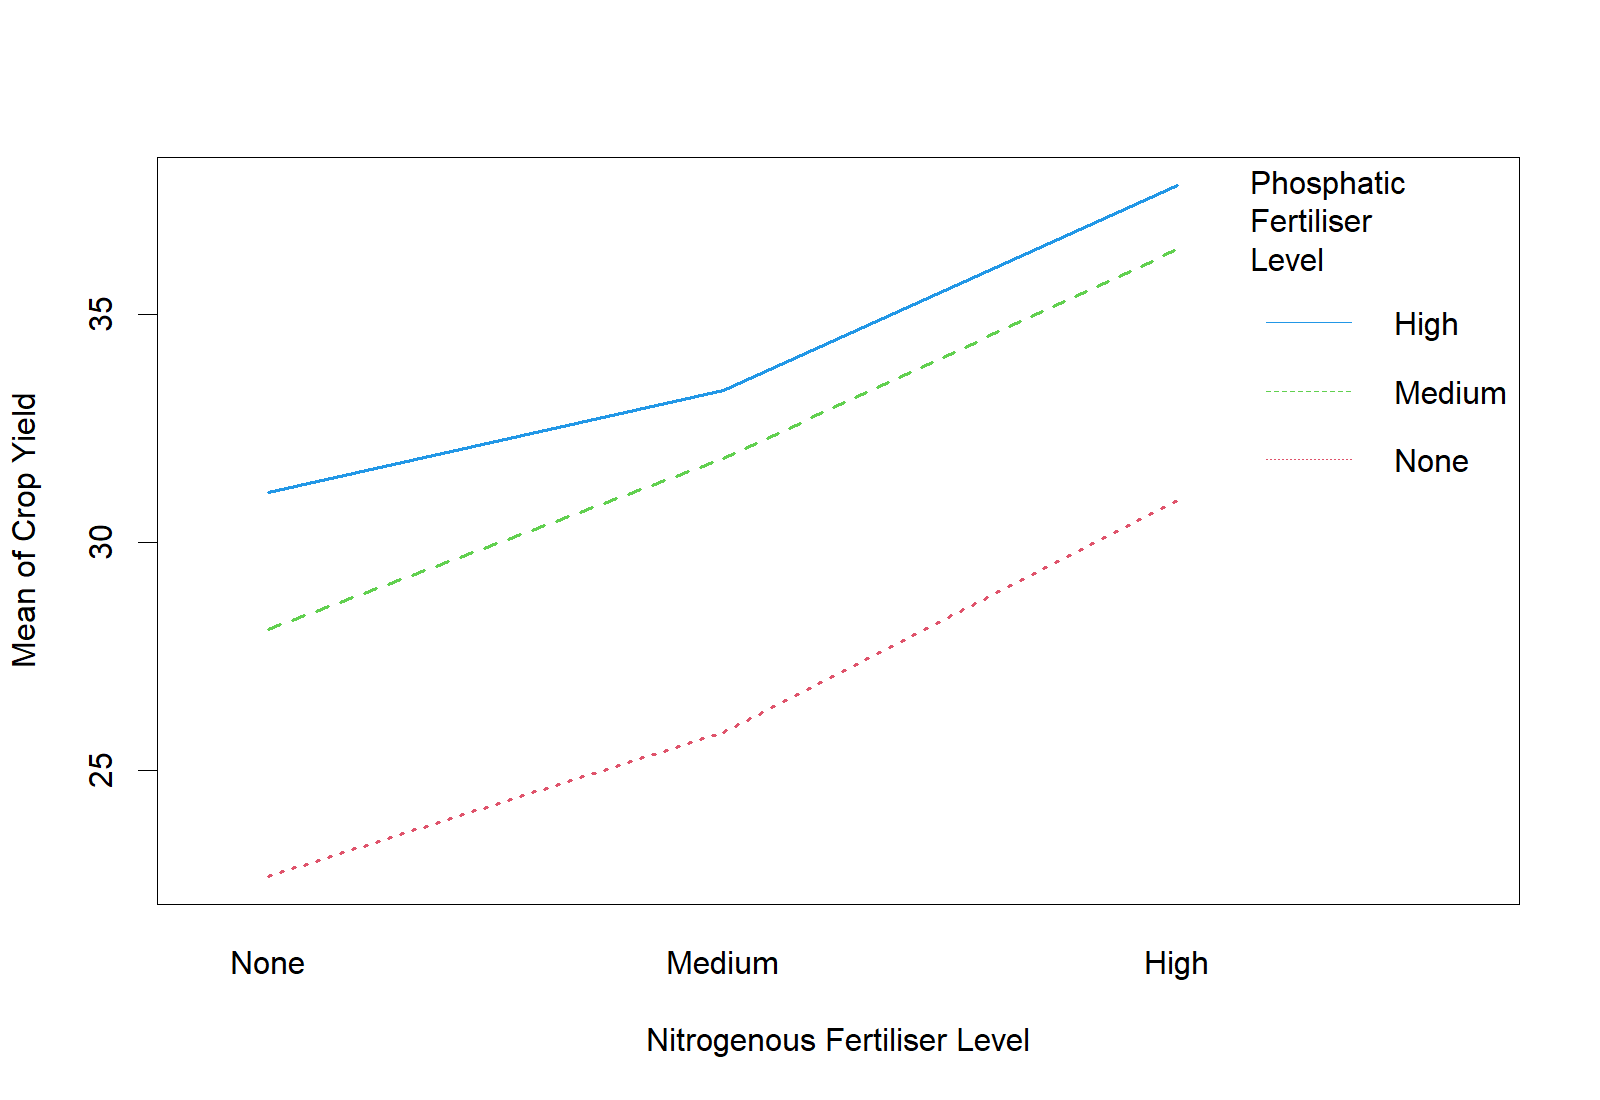
\includegraphics[width=\linewidth]{Figures/Interaction Plot (Nitrogenous).png}
    \caption{Interaction Plot (Nitrogenous)}
\end{figure}

\begin{figure}[ht]
    \centering
    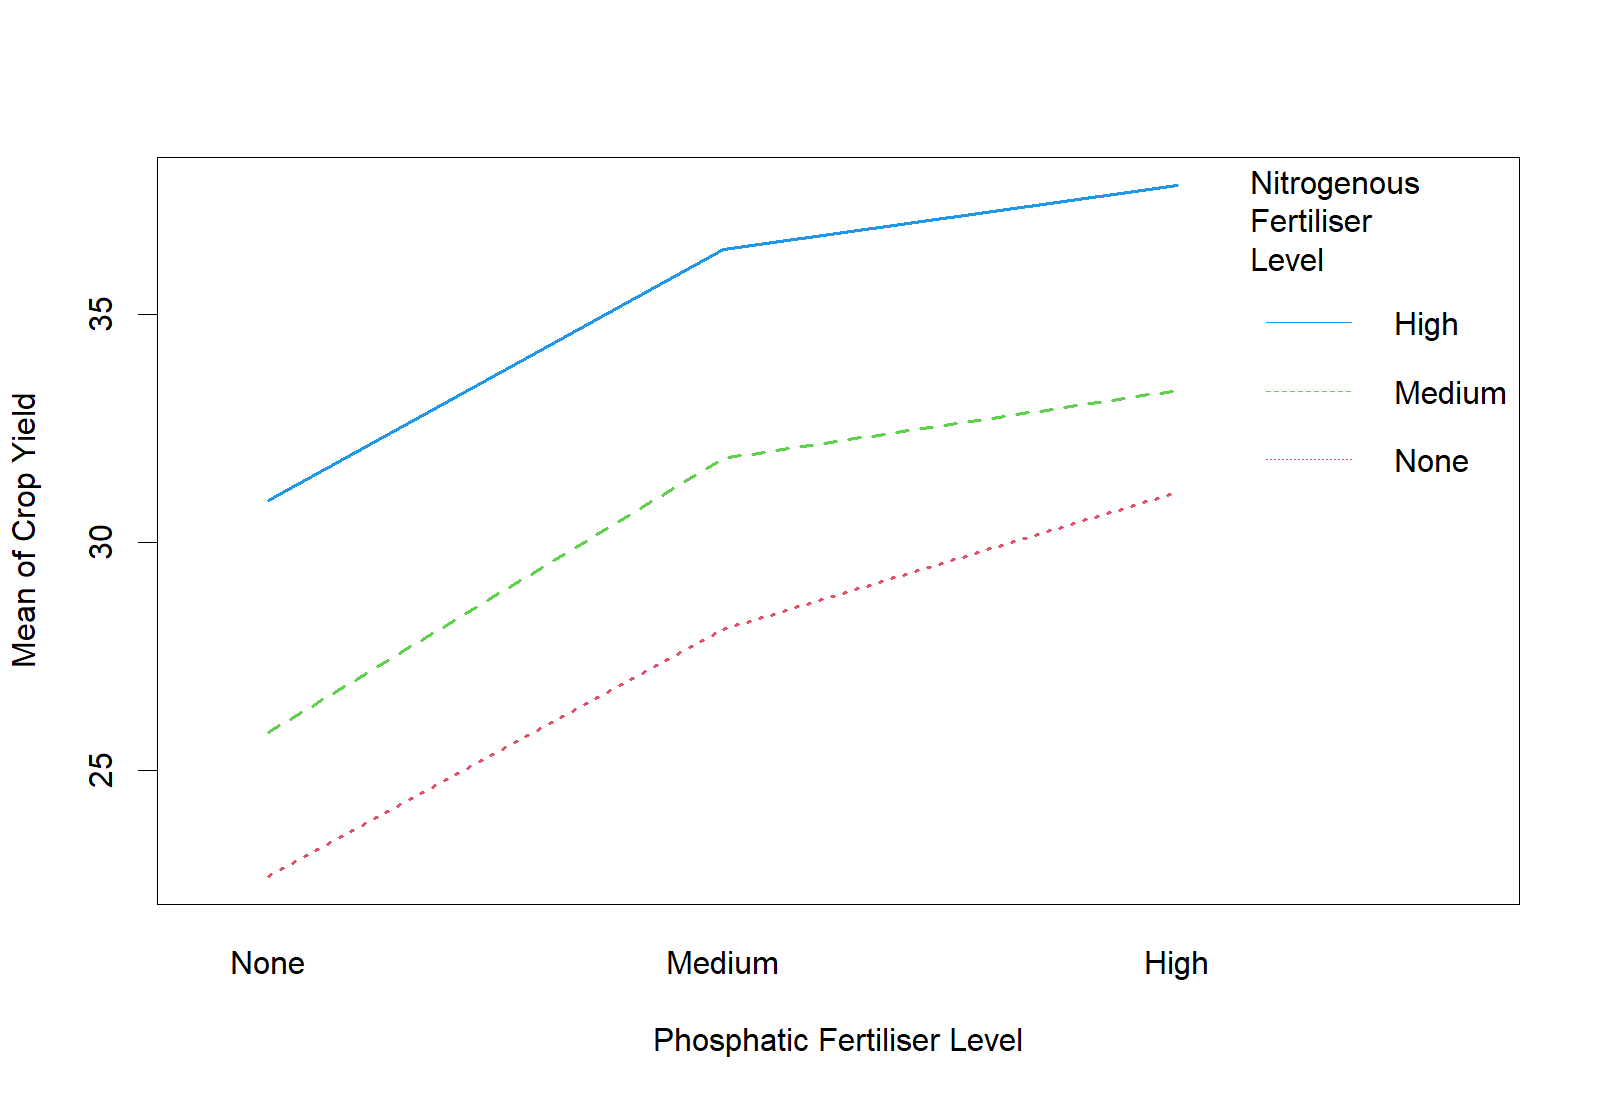
\includegraphics[width=\linewidth]{Figures/Interaction Plot (Phosphatic).png}
    \caption{Interaction Plot (Phosphatic)}
\end{figure}

\begin{figure}[ht]
    \centering
    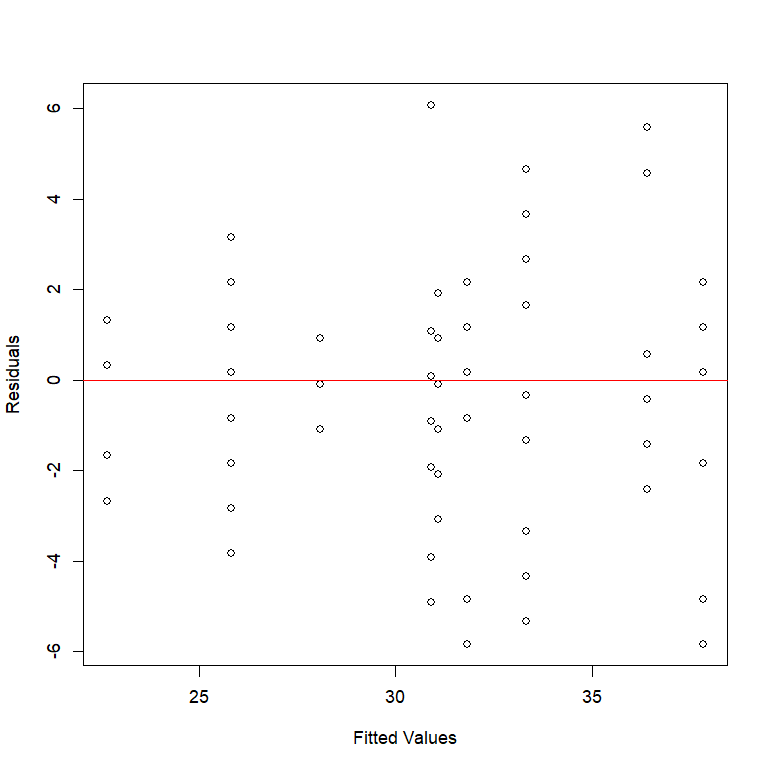
\includegraphics[width=0.8\linewidth]{Figures/Residual vs Fitted.png}
    \caption{Residuals vs Fitted Values Plot}
\end{figure}

\begin{figure}[ht]
    \centering
    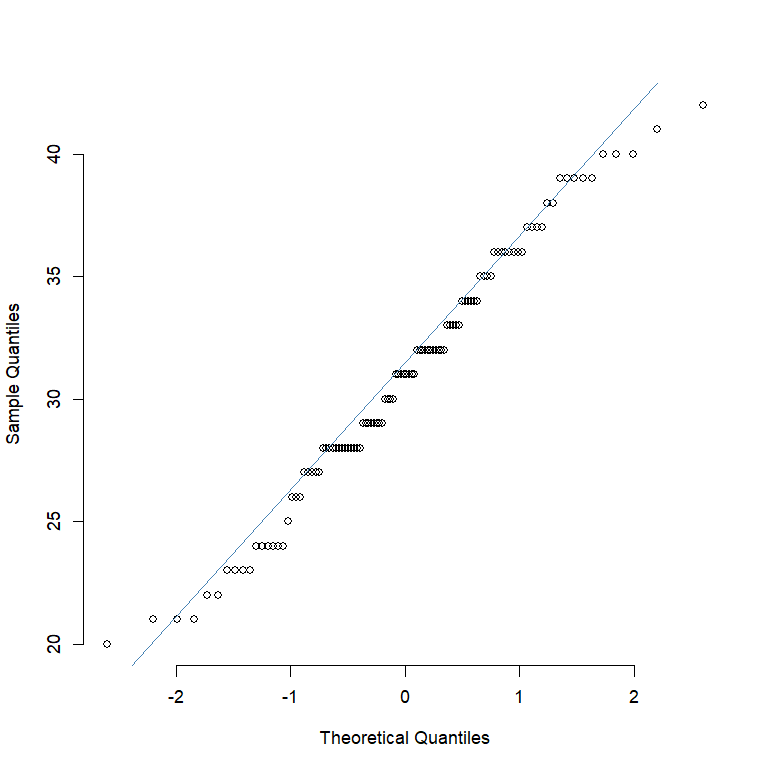
\includegraphics[width=0.8\linewidth]{Figures/Q-Q Plot.png}
    \caption{Normal Q-Q Plot}
\end{figure}


\section{Discussion}

Table 2 shows the results from conducting an ANOVA test on the data in R.
The $p$-values corresponding to the effect of N and P individually on crop yield is less than 2e-16.
This is far less than the required significance level of $0.05$, so can therefore reject $H^1_0$ and $H^2_0$.
This confirms that the results from previous studies about these chemicals individually do hold true in the context of \textit{The Islands}.

However, we observe that the ANOVA test for the interaction between N and P resulted in a $p$-value of 0.7537.
This is greater than the required significance level of 0.05.
Hence, the evidence is not strong enough and we fail to reject $H^3_0$.

This is also supported by the interaction plots for N and P in Figures 1 and 2 respectively.
Both plots show that there is little to no variation in the gradient between the different levels of the other nutrient.
Therefore, the visual evidence supports the decision to fail to reject $H^3_0$ based on this test.

By using a two way ANOVA test statistic for this experiment, we assumed that
$\epsilon_{ijk}$ are independent and normally distributed around 0.
Figure 3 clearly shows visually that the mean for this distribution was 0.
Also, Figure 4 visually confirms the assumption of being normally distributed. Therefore, this assumption was valid and is supported by the experimental data.

\subsection{Limitations}

A limitation with this experiment is that the crops were only given two days to grow due to time constraints.
This possibly means that the crops did not have enough time to fully grow before they were harvested, which would affect the validity of the data collection.
This is due to the possibility of an interaction between N and P occurring after 2 days.
In a future experiment, the growth of crops could be measured in intervals over a longer time span to see how the two chemicals interact over some longer time span.

\section{Conclusion}

This statistical experiment aimed to investigate the effect of N and P on expected crop yield as well as the interaction between them.
After collecting data and performing a two-factor ANOVA test, we rejected $H^1_0$ and $H^2_0$ confirmed the individual relationships between N and P and crop yield.
However, based on the collected data, there wasn't enough evidence to reject $H^3_0$ and hence we could not confirm any interaction between the two chemicals.


\newpage

\printbibliography

\newpage

\appendix

\begin{table}[ht]
    \centering
    \caption{Two-factor ANOVA table}
    \begin{tabular}{cccccc}
    \hline
    \makecell{Source\\ of Variation} & \makecell{Degrees\\ of Freedom} & \makecell{Sum\\ of Squares} &  \makecell{Mean\\ of Squares} & F value & \(P(f > F)\)\\ \hline
    Nitrogenous & 2 & 1105.56 & 552.78 & 89.7131 & \(<\)2e-16\\
    Phosphatic & 2 & 1123.39 & 561.69 & 91.1602 & \(<\)2e-16\\
    Interaction & 4 & 11.72 & 2.93 & 0.4756 & 0.7535\\
    Error & 99 & 610.00 & 6.16\\ \hline
    \end{tabular}
\end{table}

No AI was used in the making of this report.\\
Links to document version history:\\
\hspace*{1em} \url{https://github.com/Hyeoni77/STAT1301-Research-Project}

\newpage

Screenshots of Overleaf History:
\begin{figure}[ht]
    
\includegraphics[width=0.08\linewidth]{History/History 1.png}
    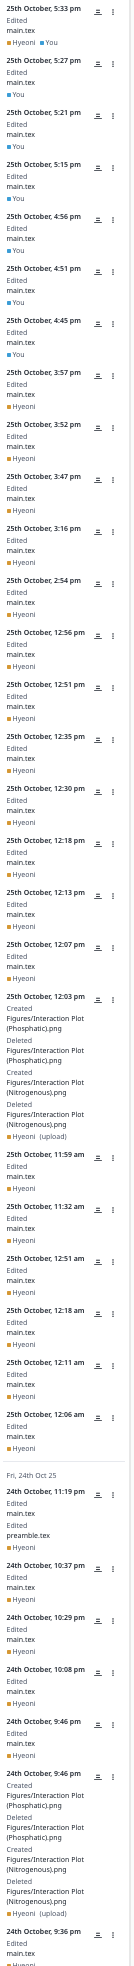
\includegraphics[width=0.08\linewidth]{History/History 2.png}
    
\includegraphics[width=0.08\linewidth]{History/History 3.png}
    
\includegraphics[width=0.08\linewidth]{History/History 4.png}
\end{figure}
\end{document}